\subsection{Pilot Results}
\label{sec:result}

\noindent Our pilot results focus on two things: First, what is the impact of unfair treatment in general, and second, what is the impact of unfair treatment in specific micro-climates.


\paragraph{Unfair treatment in general:} We found short-term impacts of discrimination on mental health and behavior. We explore this longitudinally, meaning we look at Exposure to discrimination on the day of (day 0) and response variables (health and behavior) on day 1, day 2 and so on.  We found that discriminatory encounters show strong (high confidence) relationships with same-day and next-day daily reports of depression and frustration (\textit{p} $<.001$), but not positive affect.  This is consistent with earlier reports that discrimination is more strongly associated with higher negative but not lower positive states \cite{Schmitt:2014}. 
The psychological distress we observe in our participants is stronger on the day of unfair treatment than the day after (larger $\beta$'s). We furher examined the associations on the following days and the distress returns to values similar to those in the control group (people who did not report unfair treatment) on the second day (\fig{fig:results-affect-dieoff}). When we look at the whole study, we  find that although the immediate impact of unfair treatment fades quickly, people who report unfair treatment \textit{and} score lower on social support, report higher levels of depression (%\fig{fig:results-discrimiantionXsocial}, (
$\beta$ = -0.15, p-value=0.027). This is aligned with differential reactivity hypothesis for the impact of unfair treatment as also reported elsewhere (\eg \cite{Mossakowski:2014}): having social support buffers some of the psychological distress of unfair treatment. This significant buffering effect, uniquely attributable to discrimination, suggests promising directions for program support and interventions. 

\begin{figure}
     \centering

\begin{subfigure}[t]{0.49\textwidth}
%    \small
    \centering
    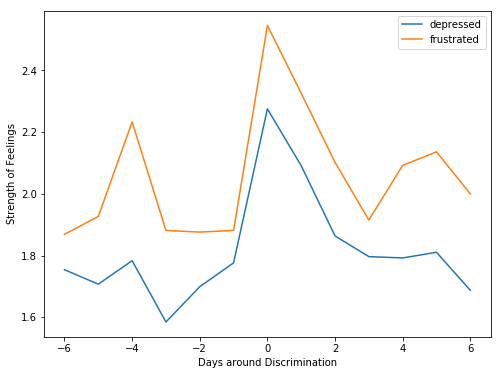
\includegraphics[width=\textwidth]{img/affect-beforeafter.png}
    \caption[Affect ratings before and after unfair treatment]{Ratings of feeling depressed and frustrated (1: not at all, 5: extremely) 6 days before and after reports of unfair treatment. Day of unfair treatment is at zero. The following days come on the right as positive numbers and the days before come on the left as negative numbers. There is a large peak on the day of the report which lasts an additional day but then more or less dies off.
    }
    \label{fig:reeults-affect-dieoff}
\end{subfigure}
\hfill
\begin{subfigure}[t]{0.49\textwidth}
    \centering
    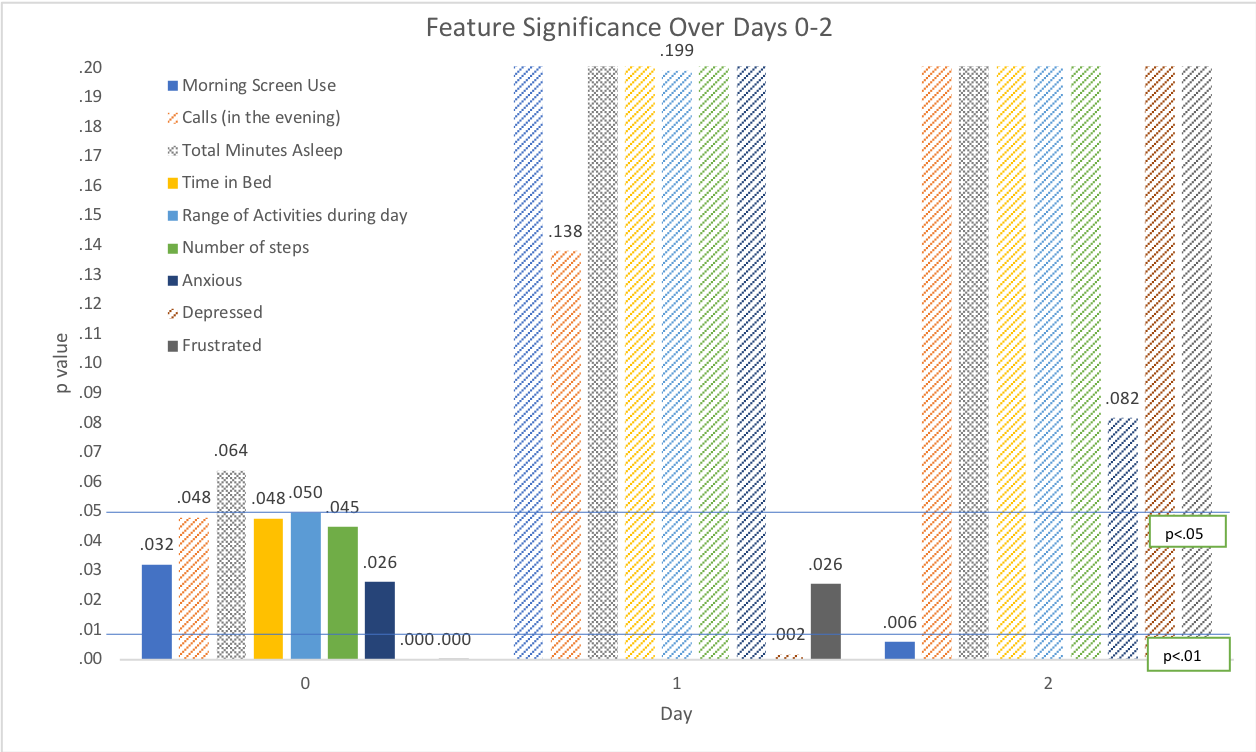
\includegraphics[width=\textwidth]{img/feature-significance}
    \caption[Feature significance over time]{Patterns of feature significance within two days of the discrimination event. The shortest bars represent the highest significance values (\eg Depressed and Frustrated on day 0; Depressed on day 1; Morning screen use on day 2) Most of short-term relations exist on the day of the event and a few on the next day.  Lines are shown at p<.05 and p<.01.}
    \label{fig:die-off}
\end{subfigure}

\end{figure}

These changes in affect also translate into behavior: people walk more (by $\sim$500 steps), have more evening calls ($\sim$1 more), interact more with their phone in the morning ($\sim$5 more interactions), and spend less time in bed ($\sim$15 minutes less).
To explore the reduction in these effects over time, we looked at a group of 6 of the most predictive variables found in our analysis. We calculated the confidence (\textit{p}-value) that these variables would be different in people reporting discrimination and those not reporting discrimination % with which these could be associated with discrimination for 
on day 0, day 1, and day 2 following the discrimination event. We also add in self-reported affect ratings that showed significant relations. Our results (shown in Figure~\ref{fig:die-off}) demonstrate that most to all of the impact found in our data occurs on  day 0 (day of)  the discrimination. This effect then reduces (\textit{p}-values rise) within the next two days. \jm{Yasaman: need corrected chart!}

\paragraph{Impact of microclimate and other moderators on unfair treatment:} \jm{xx to fill out. There was very old data in the proposa}
In the chart below, the Y axis shows the percentage of engineers who were at risk on each scale in January (start of study) and June (end of study) of 2018. We choose to focus on engineers in order to compare engineers enrolled in protective micro-climates from their peers who do not share the same protective factors. These micro-climates are the Direct Admit program, in which students are directly admitted to the major and do not have to compete for admission to an engineering department; and the STARS program, which is an onboarding program for first-generation college students, and students from low-income backgrounds and high-poverty high schools in Washington; these students tend to struggle in engineering programs because they  might not be fully prepared for their prerequisite  courses. 
